\chapter{Fortran90の基礎5〜より高度な数値計算に向けて〜}
\section{配列}
\lstinputlisting[caption={ベクトルの内積. }, label=dotproduct]{source/3/Subroutine0.f90}

\lstinputlisting[caption={行列の和. }, label=matrixsum]{source/3/MatrixSum.f90}

\subsection*{$<$演習課題$>$}
適当な数列を読み込み, その平均値と標準偏差を計算するプログラムを作成せよ.

\section{サブルーチン}
ソースコード\ref{dotproduct}のうち,
内積計算のように汎用性のある部分は独立した副プログラム(サブルーチン)として分けて記述するのがよい.
以下にサブルーチンDotProductとそれを呼び出すメインプログラムの例を示す.
\lstinputlisting[caption={ベクトルの内積. }, label=subroutine]{source/3/Subroutine.f90}
上の例のように数十行程度の短いプログラムの場合にはあえてサブルーチン化する利点は感じられないかもしれないが,
同じ処理を繰り返し実施する場合や,
数千, 数万行にも及ぶ長いプログラムを作成する場合にはサブルーチン化は必須の技術となる.


\subsection*{$<$演習課題$>$}
三次元ベクトル$\bm{a}, \bm{b}$の成分を入力し, それらの外積
\begin{equation}
\begin{pmatrix}
a_1 \\ a_2 \\ a_3
\end{pmatrix}
\times
\begin{pmatrix}
b_1 \\ b_2 \\ b_3
\end{pmatrix}
=
\begin{pmatrix}
a_2b_3-a_3b_2 \\ a_3b_1-a_1b_3 \\ a_1b_2-a_2b_1
\end{pmatrix}
\end{equation}
を計算するプログラムを作成せよ.
外積の計算部分はサブルーチン化せよ.
%\lstinputlisting[caption={繰り返し処理. }, label=doloop]{source/3/CrossProduct.f90}

\subsection*{$<$演習課題$>$}
三次元ベクトル$\bm{a}, \bm{b}, \bm{c}$の成分を入力し, ベクトル三重積
\begin{equation}
(\bm{a} \times \bm{b}) \times \bm{c}
\end{equation}
を計算するプログラムを作成せよ.
また, ベクトル三重積の公式,
\begin{equation}
(\bm{a} \times \bm{b}) \times \bm{c} = (\bm{a} \cdot \bm{c})\bm{b} - (\bm{b} \cdot \bm{c})\bm{a}
\end{equation}
の右辺を計算し, 等号が成り立っていることを確認せよ.
%\lstinputlisting[caption={繰り返し処理. }, label=doloop]{source/3/VectorTripleProduct.f90}

%\lstinputlisting[caption={繰り返し処理. }, label=doloop]{source/3/Inverse2D.f90}
%\lstinputlisting[caption={繰り返し処理. }, label=doloop]{source/3/MatrixVector.f90}
%\lstinputlisting[caption={繰り返し処理. }, label=doloop]{source/3/MatrixProduct.f90}


\section*{その他書きたいこと}
\begin{enumerate}
\item parameter文
\item exit文(doループを抜けるとき)
\item goto文(多重ループを抜けるときだけ)
\item 継続行の書き方
\item 無限ループの書き方
\item gnuplotで絵が描けるような課題を増やしたい
\end{enumerate}

\chapter{数値計算への応用}
\section{漸化式}
\begin{enumerate}
\item 等差数列
\item 階差数列
\end{enumerate}
など簡単な漸化式のサンプルプログラムと演習問題.

\section{Mandelbrot集合}
Mandelbrot集合とは,
\begin{equation}
z_{n+1}=z_n^2+c, \ \ \ z_0=0
\end{equation}
という漸化式で定義される複素数列$z_n$が$n \to \infty$の極限で発散しないという
条件を満たす複素数$c$の集合である.
Mandelbrot集合はその一部が全体と相似であり, フラクタルと呼ばれる.

$|z_n|>2$のとき, $|z_{n+1}/z_n|>1$となることが示されるので(証明略),
複素数列が発散する条件はある$N$に対して$|z_N|>2$となることである.

\begin{figure}[ht]
\centering
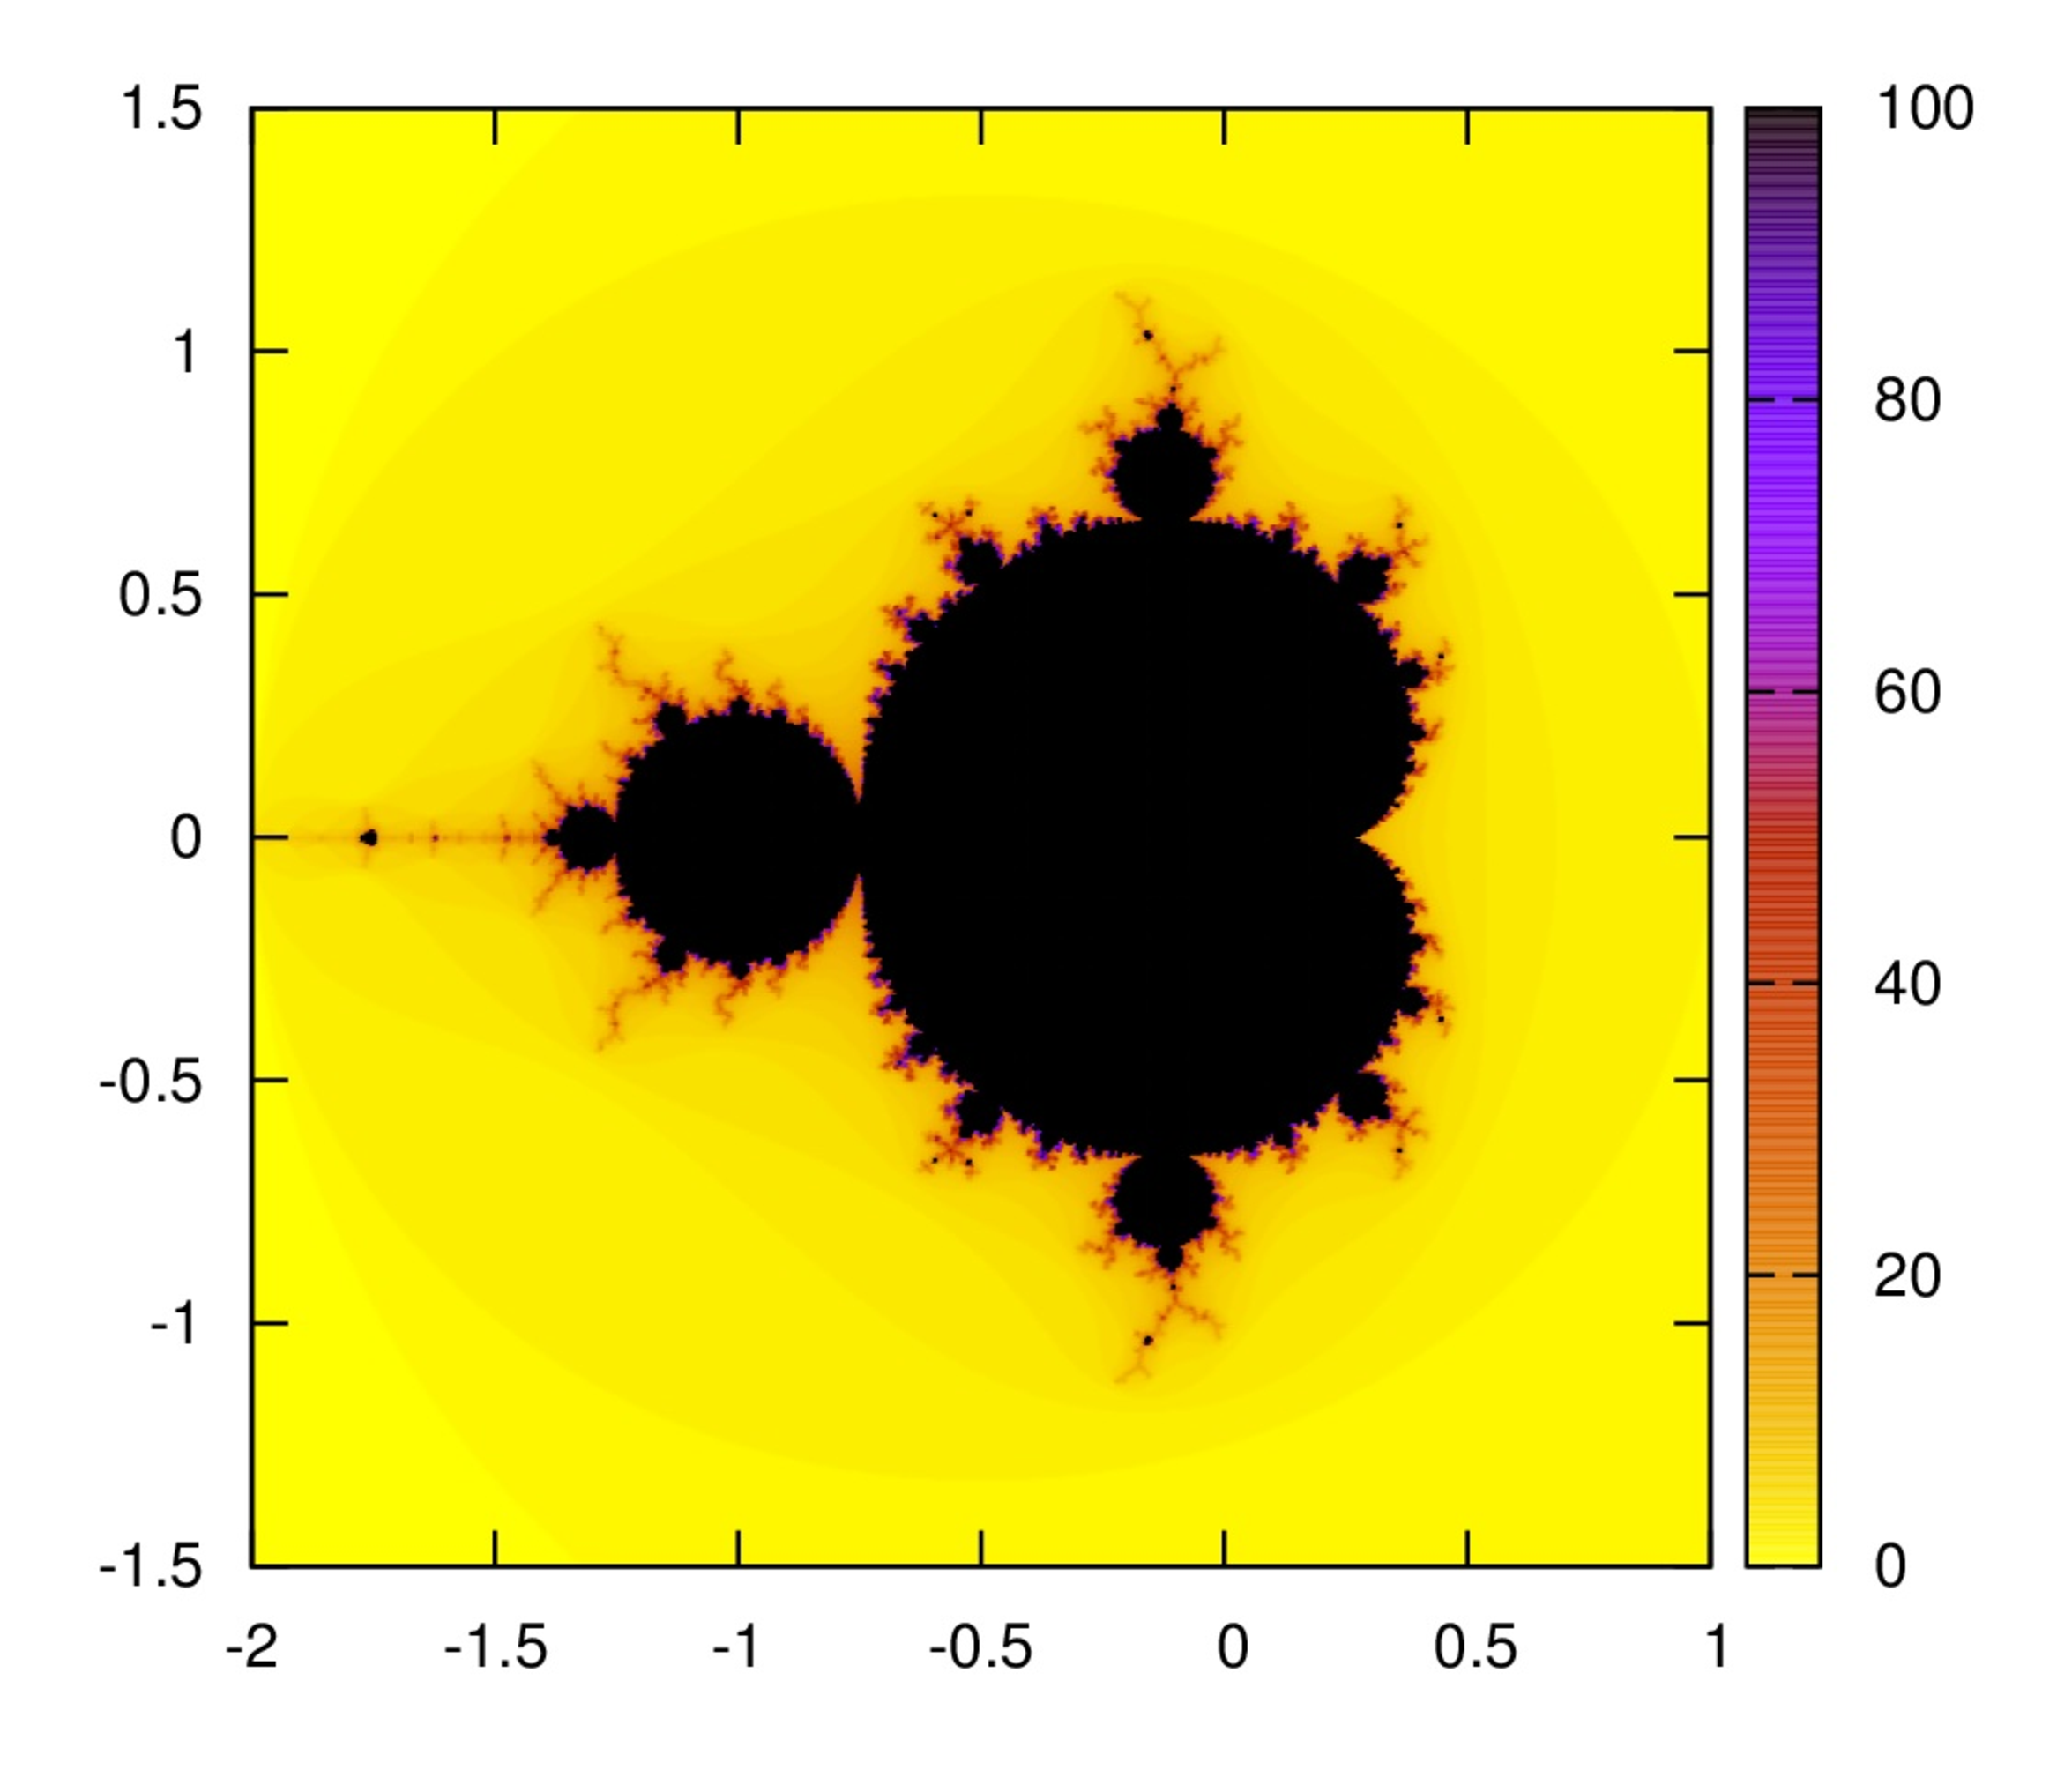
\includegraphics[width=0.75\linewidth]{source/figure/mandel}
\caption{Mandelbrot集合. }
\end{figure}

\subsection*{$<$演習課題$>$}
\begin{enumerate}
\item 複素数$c$を与え, $|z_N|>2$を満たす最初の$N$を出力するプログラムを作成せよ.
\item 上のプログラムを改造して, $-2 \le \Re[c] \le 1, -1.5 \le \Im[c] \le 1.5$の範囲における$N$をファイルに出力せよ.
また, 出力ファイルをカラーマップで描画せよ.
\item 図形の一部を解像度を上げて再計算し, Mandelbrot集合がフラクタルであることを確かめよ.
\end{enumerate}

\section{常微分方程式}
一階の微分方程式
\begin{equation}
\frac{dx}{dt}=f(x,t)
\end{equation}
を数値的に解くことを考える.
計算機は離散的な値しか扱うことができないので, 微分方程式を差分方程式に近似する.
その最も単純な近似が次のEuler法である.
\begin{equation}
\frac{x_{n+1}-x_{n}}{\Delta t}=f(x_n,t_n).
\end{equation}
ここで, $\Delta t$を十分に小さい時間刻み幅として,
第$n$ステップにおける$t, x$をそれぞれ$t_n(=n \Delta t), x_n$としている.
初期条件$x(0)=x_0$を与えた上で, $n=0, 1, 2, \cdots$に対して
\begin{equation}
x_{n+1}=x_{n}+f(x_n,t_n)\Delta t
\end{equation}
として逐次$x_n$を求めていく. なお, Taylor展開により,
\begin{equation}
\begin{split}
x(t+\Delta t)&=x(t)+\frac{dx}{dt}(t)\Delta t+O(\Delta t^2)\\
&=x(t)+f(x,t)\Delta t+O(\Delta t^2)
\end{split}
\end{equation}
であるから, Euler法では1ステップあたり$\Delta t^2$程度の誤差が生じることになる. \\

常微分方程式
\begin{equation}
\frac{dx}{dt}=ax, \ \ \ x(0)=1
\end{equation}
を数値的に解く. なお, この方程式の解は
\begin{equation}
x(t)=\exp(at)
\end{equation}
で与えられる.

\lstinputlisting[caption={Euler法. }, label=eulermethod]{source/5/EulerMethod.f90}

\subsection*{$<$演習課題$>$}
ここに, Euler法の適当な演習課題を一つ追加.
$\Delta t$を変えたらどうなるか確かめてみる.

\section{Lorenz方程式}
気象学者のLorenzは1963年に熱対流の近似モデルとして
以下の方程式を提案した(Lorenz方程式).
\begin{equation}
\dfrac{dx}{dt}=-ax+ay,
\end{equation}
\begin{equation}
\dfrac{dy}{dt}=\mu x-y-xz,
\end{equation}
\begin{equation}
\dfrac{dz}{dt}=-bz+xy.
\end{equation}
Lorenzは数値計算により, この方程式の解が
不規則で周期性をもたない振動をすることを発見した.
このような非周期運動は現在ではカオスと呼ばれている.

なお, Lorenz方程式は自明解$x=y=z=0$の他に,
$\mu >1$のとき, 解$x=y=\pm \sqrt{b(\mu-1)}, z=\mu-1$をもつ.

\begin{figure}[ht]
\centering
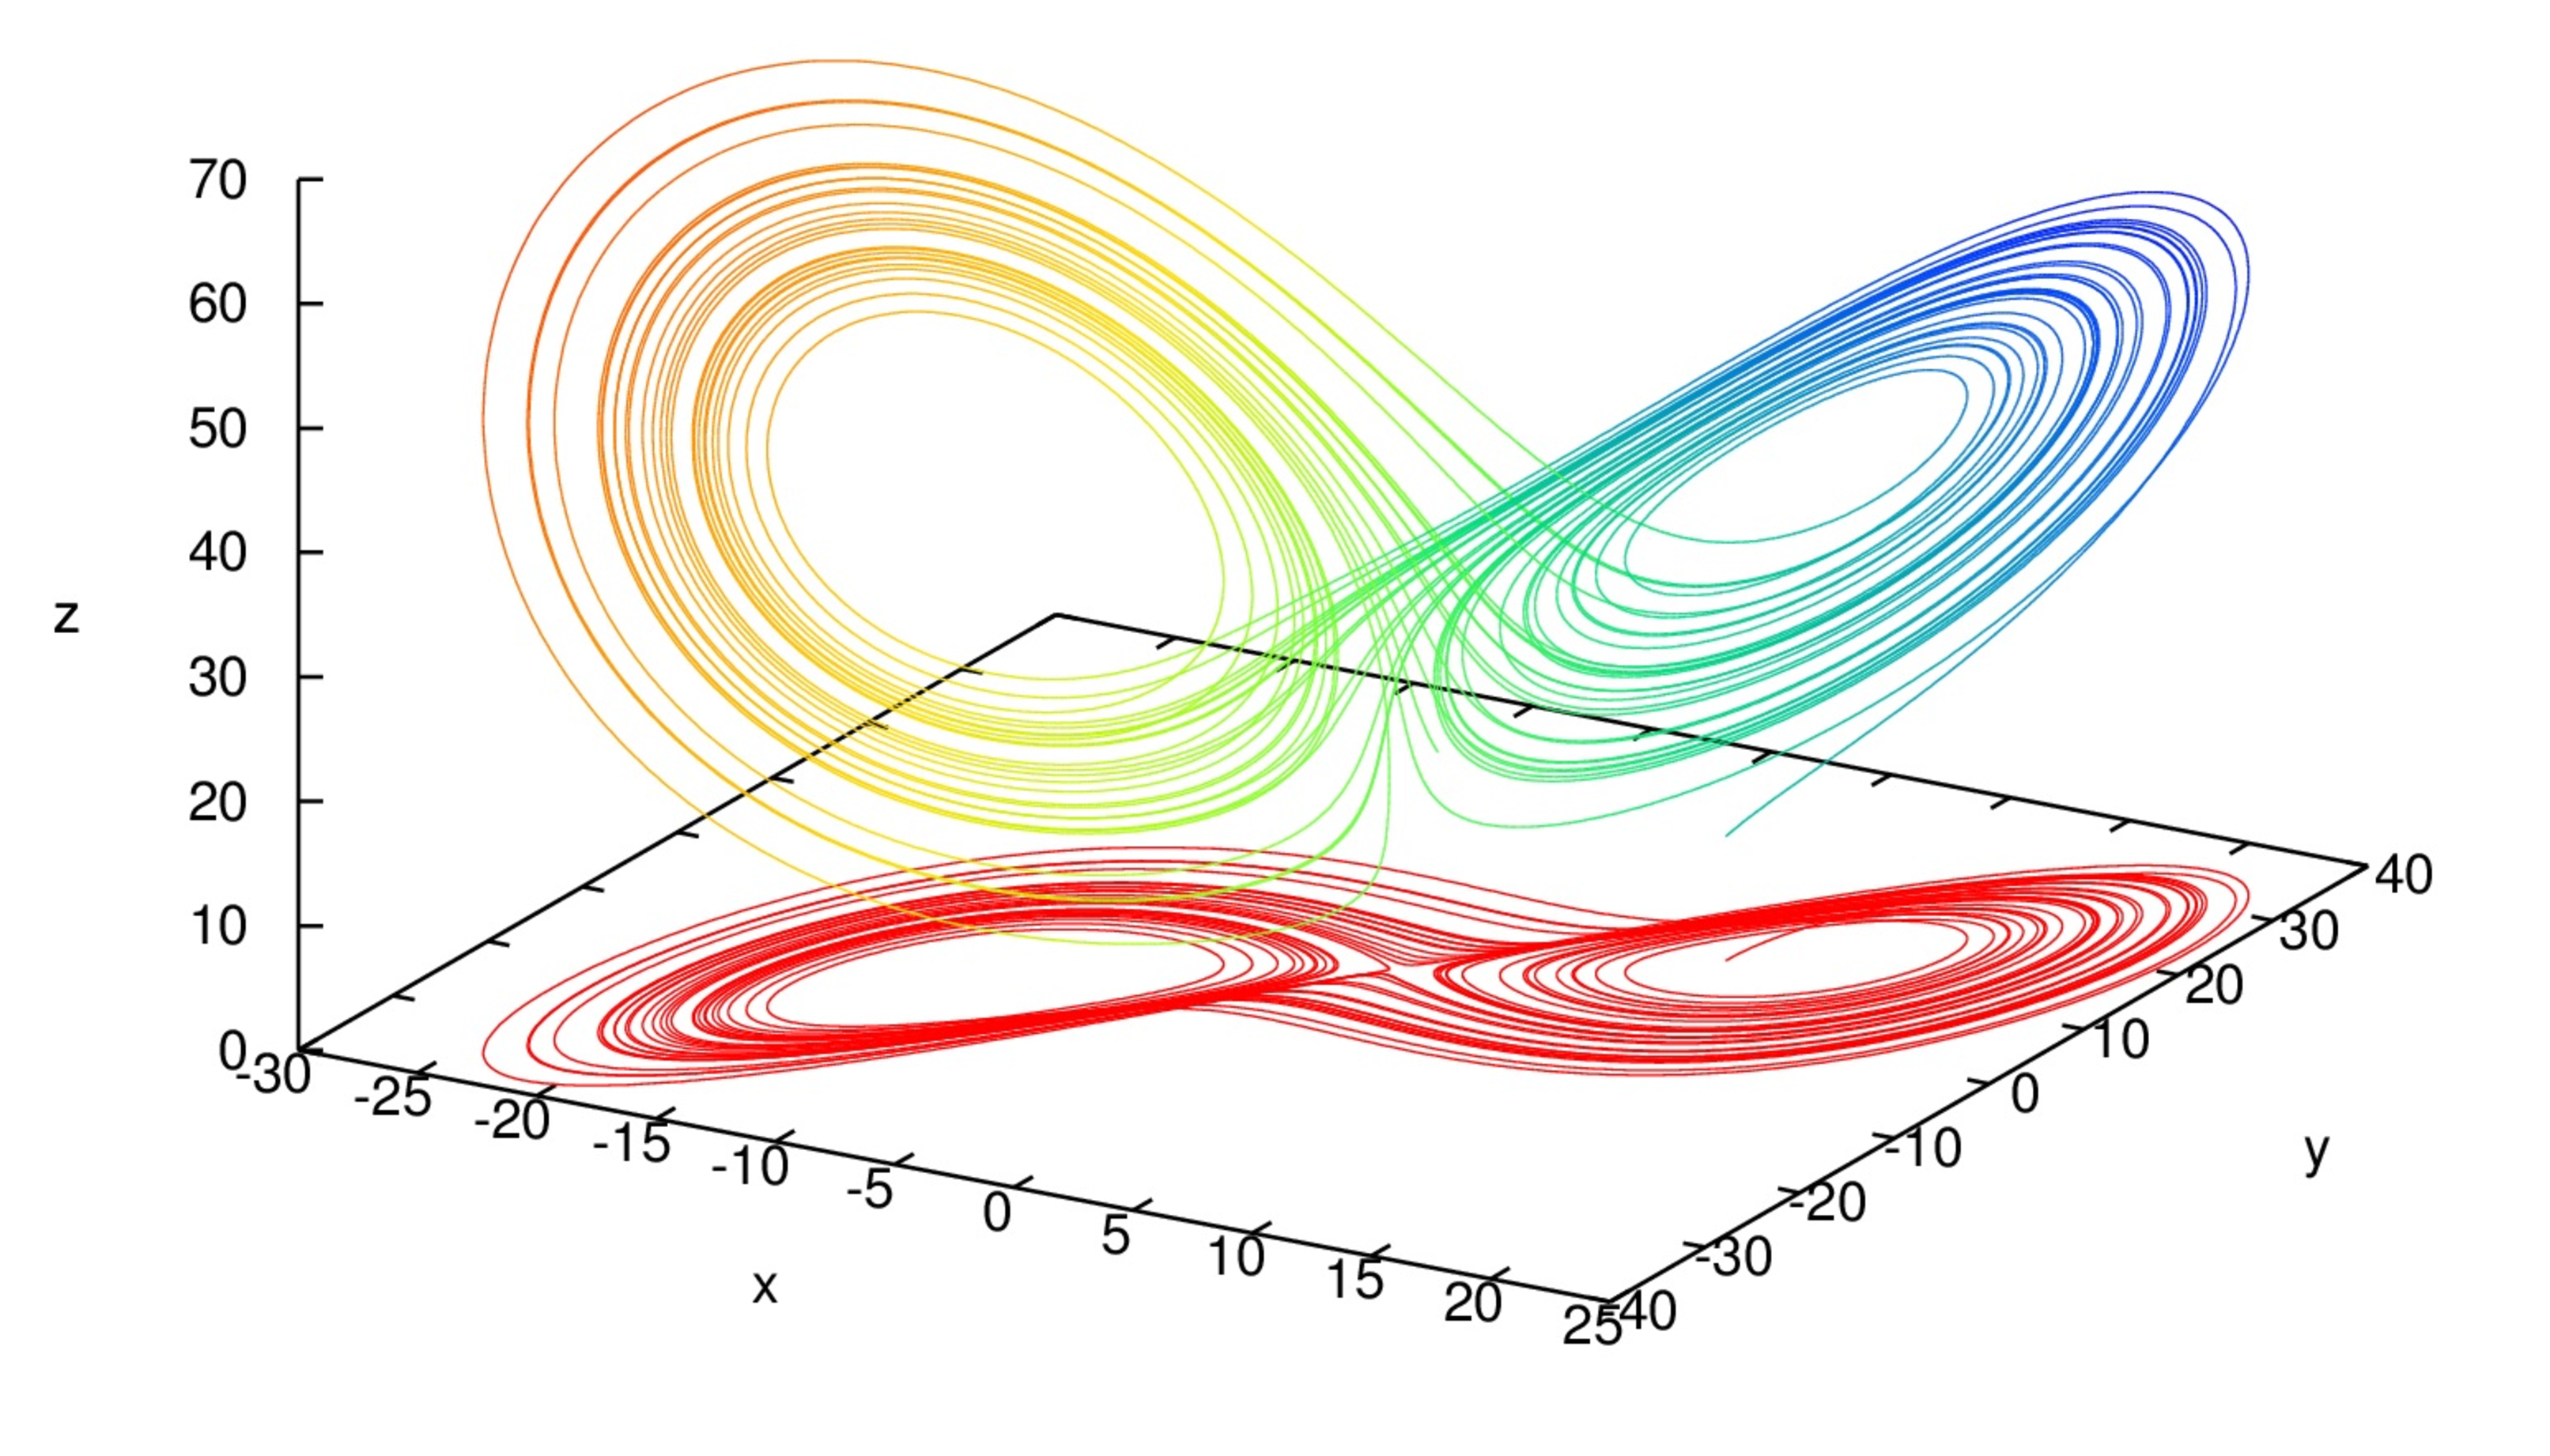
\includegraphics[width=0.9\linewidth]{source/figure/lorenz.eps}
\caption{Lorenzアトラクター. }
\end{figure}

\subsection*{$<$演習課題$>$}
\begin{enumerate}
\item $a=10, b=8/3$と固定した上で, Lorenz方程式のシミュレーションを実施せよ.
$\mu$を徐々に増加させ, どのような解が現れるか調べよ.
\item 初期値がわずかに(例えば1\%程度)異なる2ケースのシミュレーション結果を比較せよ.

\end{enumerate}


\section{運動方程式}
質点の自由落下をシミュレーションする.
質点の質量を$m$, 重力加速度を$g$, 初期位置を$h$, 初速を$u_0$とする.
鉛直座標として$x$をとると, 運動方程式は
\begin{equation}
m\frac{d^2x}{dt^2}=-mg, \ \ \ x(0)=h, \ \ \ \frac{dx}{dt}(0)=u_0
\label{eq_freefall}
\end{equation}
で与えられ, その解は次で与えられる.
\begin{equation}
x(t)=h+u_0t-\frac{1}{2}gt^2.
\end{equation}

式(\ref{eq_freefall})を以下のように変形することで一階の連立微分方程式が得られる.
\begin{equation}
\frac{dx}{dt}=u, \ \ \ x(0)=h,
\end{equation}
\begin{equation}
\frac{du}{dt}=-g, \ \ \ u(0)=u_0.
\end{equation}
これをEuler法を用いて数値的に解けばよい.
プログラムの例を以下に示す.
\lstinputlisting[caption={質点の自由落下シミュレーション. }, label=freefall]{source/6/FreeFall.f90}



続いて, 質点が空気抵抗を受ける場合のシミュレーションをおこなってみよう.
質点の投射方向は鉛直方向に限定しない(すなわち, 斜方投射).
以後, $x, y$をそれぞれ水平, 鉛直方向の座標とする.


球形物体に働く空気抵抗の大きさ$D$は一般に物体の速さ$(U=\sqrt{(dx/dt)^2+(dy/dt)^2})$の二乗に比例するとしてモデル化される:
\begin{equation}
D=\frac{1}{2}\rho U^2 \pi a^2 C_D.
\end{equation}
ここで, $\rho$は空気の密度, $a$は球の半径である.
また, 抗力係数$C_D$はReynolds数$Re=2aU/\nu$ ($\nu$は空気の動粘性係数)
と呼ばれる無次元数の関数であり,
$5 \times 10^2 < Re < 1 \times 10^5$のとき約0.44で一定であることが知られている.

空気抵抗は速度と逆向きに働くので, これを成分$(D_x, D_y)$に分けて運動方程式を書くと,
\begin{equation}
m\frac{d^2 x}{dt^2}=-D_x,
\end{equation}
\begin{equation}
m\frac{d^2 y}{dt^2}=-mg-D_y,
\end{equation}
\begin{equation}
D_x=\frac{dx/dt}{\sqrt{(dx/dt)^2+(dy/dt)^2}}D=\frac{1}{2}\rho \pi a^2 C_D\sqrt{\Big(\frac{dx}{dt}\Big)^2+\Big(\frac{dy}{dt}\Big)^2}\frac{dx}{dt},
\end{equation}
\begin{equation}
D_y=\frac{dy/dt}{\sqrt{(dx/dt)^2+(dy/dt)^2}}D=\frac{1}{2}\rho \pi a^2 C_D\sqrt{\Big(\frac{dx}{dt}\Big)^2+\Big(\frac{dy}{dt}\Big)^2}\frac{dy}{dt}.
\end{equation}
となる.

\if0 %%%%%%%%%%%%%%%%%%%%%%%%%%%%%%%%%%%%%%%%%%%%%%%%%%%%%%%%%%%%%%%
\subsection{Reynolds数が小さい場合}
$Re<0.1$のとき, 抗力係数は理論的に
\begin{equation}
C_D=\frac{24}{Re}
\end{equation}
となることが知られている.

このとき, 運動方程式は
\begin{equation}
m\frac{d^2 x}{dt^2}=-6\pi \rho \nu a \frac{dx}{dt},
\end{equation}
\begin{equation}
m\frac{d^2 y}{dt^2}=-mg-6\pi \rho \nu a \frac{dy}{dt},
\end{equation}
となり, 抵抗は速さの一乗に比例する.
比例係数$6\pi \rho \nu a$は物性値と球の大きさによって決まる.

\begin{table}[h]
\centering
\begin{tabular}{ccc}
\hline
パラメータ & 値 & 備考 \\
\hline
質量$m$ [kg] & - & 適当に与える \\ \hline
半径$a$ [m] & - & 適当に与える \\ \hline
重力加速度$g$ [m/s$^2$] & 9.80665 & - \\ \hline
空気の密度$\rho$[kg/m$^3$] & 1.261 & 280Kの場合 \\
 & 1.176 & 300Kの場合 \\ \hline
空気の動粘性係数$\nu$[m$^2$/s] & 1.395 $\times 10^{-5}$ & 280Kの場合 \\
 & 1.579 $\times 10^{-5}$ & 300Kの場合 \\ \hline
水の密度$\rho$[kg/m$^3$] & 9.999 $\times 10^2$ & 280Kの場合 \\
 & 9.966 $\times 10^2$ & 300Kの場合 \\ \hline
水の動粘性係数$\nu$[m$^2$/s] & 1.436 $\times 10^{-6}$ & 280Kの場合 \\
 & 8.574 $\times 10^{-7}$ & 300Kの場合 \\ \hline
Reynolds数$Re$[-] & $\frac{2aU}{\nu}$ & 計算する \\ \hline
抗力係数$C_D$[-] & $\frac{24}{Re}$ & $Re<0.1$における理論式 \\
& $(\sqrt{\frac{24}{Re}}+0.5407)^2$ & $Re< 6000$における経験式 \\
& $0.44$ & $5 \times 10^2 < Re < 1 \times 10^5$における近似値 \\
& & (この範囲で抵抗は速度の二乗に比例) \\ \hline
スケールハイト$H_\rho$[m] & 8 $\times 10^3$ & 実際は温度によって変化する \\ \hline
\end{tabular}
\end{table}
\fi %%%%%%%%%%%%%%%%%%%%%%%%%%%%%%%%%%%%%%%%%%%%%%%%%%%%%%%%%%%%%%%%

\subsection*{$<$演習課題$>$}
\begin{enumerate}
\item 空気抵抗がない場合($C_D=0$)のシミュレーションをおこない, 解析解と比較せよ.
\item 空気抵抗がある場合のシミュレーションをおこない, 空気抵抗がない場合と比較せよ.
もしも$Re$が$5 \times 10^2 < Re < 1 \times 10^5$の範囲になければ警告メッセージを出す仕様にすること.
\item 空気の温度が変化した場合, 物体の飛距離はどのように変わるか.
\end{enumerate}

各物理量の具体的な値については, 以下の表を参考にするとよい.
\begin{table}[h]
\centering
\begin{tabular}{ccc}
\hline
パラメータ & 値 & 備考 \\
\hline
質量$m$ [kg] & - & 適当に与える \\ \hline
半径$a$ [m] & - & 適当に与える \\ \hline
重力加速度$g$ [m/s$^2$] & 9.80665 & - \\ \hline
空気の密度$\rho$[kg/m$^3$] & 1.261 & 280Kの場合 \\
 & 1.176 & 300Kの場合 \\ \hline
空気の動粘性係数$\nu$[m$^2$/s] & 1.395 $\times 10^{-5}$ & 280Kの場合 \\
 & 1.579 $\times 10^{-5}$ & 300Kの場合 \\ \hline
Reynolds数$Re$[-] & - & $2aU/\nu$ \\ \hline
抗力係数$C_D$[-] & $0.44$ & $5 \times 10^2 < Re < 1 \times 10^5$のとき \\ \hline
\end{tabular}
\end{table}



\section{素数探索}
素数とは1と自分以外に約数をもたない自然数のことである.
計算機を用いて数多くの素数を求めてみよう.

\subsection*{$<$演習課題$>$}
\begin{enumerate}
\item 適当な自然数$n$を与え, $2$から$n-1$までの自然数で割り算をおこなうことで
$n$が素数かどうかを判定するプログラムを作成せよ.
\item 上のプログラムを改造し, 10,000個の素数を探索するプログラムを作成せよ.
\item アルゴリズムを工夫して, 10,000個の素数を探索するプログラムの高速化をせよ.
もとのプログラムの何倍速くなったか.
\end{enumerate}

プログラムの実行時間の測定には, system\_clock関数を用いる.
その利用法は以下のプログラムを参照せよ.
\lstinputlisting[caption={実行時間の測定. }, label=timing]{source/7/Timing.f90}
